% Chapter 2
% Roberto Masocco <robmasocco@gmail.com>
% August 28, 2021

\chapter[Nuovi problemi e nuove soluzioni]{Nuovi problemi e nuove soluzioni}
\label{chap:Chapter2}
\doublespacing
\fontsize{14}{14}\selectfont

\newsection{Premessa}
\indent Lo sviluppo di un sistema robotico autonomo è un processo che attraversa varie fasi. Ciascuna di esse è solitamente caratterizzata dalla definizione e soluzione di problematiche inerenti diversi aspetti dell'apparato, che possono andare dalle operazioni che questo sarà chiamato a svolgere, alla sua costruzione e programmazione, fino al modo in cui i dati che esso raccoglie e che condizionano il suo funzionamento debbano essere presentati agli eventuali operatori. Volendo generalizzare dallo specifico caso applicativo, la maggior parte delle problematiche si possono ripartire tra poche tipologie di alto livello. Nonostante possa risultare controintuitivo dalla suddivisione che ci si appresta a delineare, queste non sempre si rivelano affrontabili in sequenza, né tanto meno completamente indipendenti. È anche per risolvere situazioni simili che negli ultimi tempi sono state ideate svariate tecniche di project management, volte anche a minimizzare il rischio che un errore commesso in una fase precedente possa pregiudicare quelle future, compromettendo il lavoro svolto ed allungando i tempi di sviluppo. In virtù di quanto osservato nel capitolo precedente, è chiaro che con l'aumentare della complessità dei sistemi automatici odierni e dei compiti che essi devono svolgere, queste tematiche siano quanto mai attuali. In particolare, nuovi strumenti messi a disposizione di sviluppatori e progettisti dovranno riflettere queste specificità, semplificare la gestione di situazioni tipiche dove possibile, ed evidenziare eventuali criticità per aiutare nella soluzione dei problemi. Nonostante la generalizzazione che si sta facendo possa sembrare eccessiva, nella realtà pratica si riscontra facilmente che a dispetto della varietà di casi di specie e applicazioni, le complicazioni da affrontare sono quasi sempre se non le stesse, molto simili, e lo stesso si può rilevare circa le strategie da adottare.\\
L'obiettivo di questo capitolo è presentare brevemente le problematiche che solitamente si devono affrontare quando si progetta un sistema robotico, evidenziandone le peculiarità seppur senza concentrarsi su un particolare ambito applicativo, e passare poi ad esaminare alcune recenti soluzioni hardware e software che consentono di ottimizzare il lavoro di progettazione, sviluppo e testing in loro funzione. La discussione parte ora da un livello abbastanza alto di astrazione ma diventerà via via sempre più specifica, costituendo di fatto la linea guida seguita durante il progetto che costituisce il caso di studio di questo lavoro e dunque un filo che lega tutti i capitoli successivi.

\newsection{Fasi e criticità progettuali}
\newsubsection{I task}
\indent Le prime decisioni da prendere all'inizio del progetto di un sistema automatico o robotico riguardano naturalmente le specifiche delle operazioni che questo dovrà svolgere. Esse vanno completamente delineate fin da subito nei minimi particolari, in quanto è da loro che dipenderanno tutte le scelte successive, da quelle inerenti la costruzione e la scelta dell'hardware fino alla sua programmazione. Durante questa decomposizione dei requisiti operativi in \emph{task}, intesi come singole unità di lavoro da eseguire, compariranno diversi tipi di questi ultimi. Senza scendere, per ora, nei particolari di uno specifico caso, tipologie comuni sono:
\begin{itemize}
    \item task \textbf{continuativi}, ossia iniziati all'accensione del sistema e mai interrotti fino al suo spegnimento o malfunzionamento;
    \item task \textbf{periodici}, da eseguire a intervalli regolari;
    \item task \textbf{asincroni}, svolti solo quando un particolare evento si verifica.
\end{itemize}
È facile rendersi conto di come gran parte delle funzionalità presenti nei sistemi robotici odierni possa essere decomposta in task appartenenti a ciascuna di queste categorie. Ne fanno evidentemente parte operazioni che vanno dal controllo degli attuatori, alla raccolta di dati e misure necessari agli algoritmi di controllo, fino alla comunicazione con operatori ed utenti. Le specificità di questi task avranno risvolti sia sull'hardware che dovrà realizzarli che sul software che li codificherà, i quali dovranno essere organizzati opportunamente in loro funzione, anche in modo da facilitarne lo sviluppo e la manutenzione.

\newsubsection{L'hardware}
\indent Le decisioni da prendere successivamente riguardano l'hardware da utilizzare per realizzare i primi prototipi dell'apparato. Probabilmente non si tratterà di quello che comporrà il prodotto finito, per via di eventuali errori di valutazione, imprevisti o altre problematiche sorte successivamente. Ciò nonostante esso deve essere selezionato con cura in base ai requisiti operativi, strutturali e costruttivi definiti fin qui. Le decisioni prese durante il passo precedente rivestono in questa fase un'importanza cruciale: stabilendo infatti quale sia la complessità computazionale delle operazioni che il sistema dovrà svolgere, sarà richiesto un hardware di alto livello più o meno potente, equipaggiato eventualmente con coprocessori discreti\footnote{Con il termine \emph{discreto} si intende hardware aggiuntivo montato su di un calcolatore, non in grado di operare da solo ma fatto per essere pilotato da quest'ultimo, offrendogli supporto specifico per particolari operazioni; classici esempi sono i coprocessori matematici, le GPU e le schede audio.} necessari per trattare particolari tipi di dati, o suddiviso in più sottosistemi interconnessi. Al giorno d'oggi, ricordando la dicussione fatta nel capitolo precedente circa la disponibilità di un'ampia gamma di soluzioni off-the-shelf, è d'obbligo un'indagine di ciò che offre il mercato per capire se sia possibile sfruttare componenti o SoC forniti già testati e pronti per essere utilizzati, piuttosto che ricorrere ad una soluzione proprietaria che porta generalmente con sé considerevoli costi di sviluppo, testing e validazione. Per i motivi sopracitati è molto difficile, se non impossibile, delineare fin da questo punto una struttura complessiva e definitiva dell'hardware: ciò che importa è capire di cosa c'è bisogno e se esistono sul mercato offerte compatibili con i propri requisiti, cercando di prevedere anche successive richieste aggiuntive. Seguendo questa linea, eventuali variazioni potranno essere gestite similmente con poco sforzo.\newpage
Il resto delle scelte riguardano l'hardware di più basso livello, formato in generale da:
\begin{itemize}
    \item microcontrollori veloci;
    \item attuatori;
    \item sensori;
    \item interfacce e dispositivi di comunicazione;
    \item hardware per il controllo e la supervisione;
    \item sistemi di immagazzinamento di dati.
\end{itemize}
Niente di più si può dire su di esse prescindendo dal caso di specie, tuttavia nel seguito di questo lavoro saranno descritte situazioni simili relative all'esempio che si discuterà. Per ora ci si può limitare a sottolineare che le osservazioni fatte precedentemente valgono anche per questi componenti.

\newsubsection{Il software}
\indent Eccezion fatta per quei componenti che svolgono funzioni cruciali e molto specifiche, come circuiti elettrici/elettronici, la quasi totalità delle operazioni svolte da un sistema robotico è oggi codificata in un calcolatore ad esso interno, che traduce tali istruzioni in comandi per gli altri componenti, sottosistemi, sensori o attuatori. Non è questa la sede per la discussione di procedure standard di progettazione e realizzazione del software, ma basta soffermarsi a riflettere su un punto: anche il software che governa un robot, data la complessità di quest'ultimo, avrà un'organizzazione stratificata e fortemente gerarchica. In essa, i livelli inferiori saranno occupati da quei moduli che dovranno interagire con, se non muovere, i sottosistemi più piccoli e veloci (e.g. il \emph{firmware}), e che andranno sviluppati ponendo particolare attenzione alle caratteristiche di essi ed alle loro finalità. Man mano che si sale nella scala gerarchica ci si muove verso moduli a più ampio spettro, che codificano operazioni di supervisione, pianificazione e comunicazione con gli utenti, e per questo più vicini alla nozione di software applicativo o di sistema, con cui magari si è più abituati ad avere a che fare essendo quello "maggiormente visibile" ad un utente finale. Supponendo di dover operare in questo contesto, si deve poter contare su degli strumenti che semplifichino il più possibile il design e lo sviluppo a tutti i livelli senza distinzione, aiutando nella gestione di problematiche inerenti l'organizzazione dei moduli, la comunicazione, il processamento e la memorizzazione di diversi tipi di dati.\\
Rientra in questo contesto anche una decisione circa i linguaggi di programmazione da adottare. Com'è noto, ciascuno possiede le sue caratteristiche peculiari, che ne evidenziano rispetto alle alternative punti di forza ma anche debolezze. Pochi sono i linguaggi di programmazione adatti per molteplici scopi, intendendo in questo senso il grado di facilità con cui consentono di codificare diversi tipi di task, e nessuno è da considerarsi universale. Nel seguito di questo lavoro verranno presentate, a titolo di esempio, due diverse alternative, mettendone in risalto le specificità e motivando un uso preponderante di una delle due con dei requisiti progettuali del caso di studio.\newpage

\newsubsection{I dati e le misure}
\indent Un robot, per portare a termine i propri task con successo, necessita più o meno costantemente di informazioni circa quello che gli sta accadendo intorno. Esse possono essere ricevute entro pacchetti dati, gestiti da opportune interfacce di comunicazione, oppure acquisite direttamente mediante degli organi di misurazione, comunemente detti \emph{sensori}. Per entrambe queste soluzioni, problematiche classiche che si incontrano da subito sono l'integrazione dei relativi dispositivi nel resto dell'apparato e il processamento dei dati che queste restituiscono. Esse sono peraltro cruciali, in quanto il funzionamento dell'intero apparato è quasi sempre condizionato alla possibilità di disporre di informazioni circa l'ambiente circostante e lo stato del robot stesso\footnote{Si pensi agli algoritmi di controllo in \emph{feedback}, basati sulla possibilità di acquisire misure delle azioni di controllo impartite ad un sistema e di grandezze che ne esplicitano gli effetti.}. E' dunque lecito aspettarsi che un robot sia dotato di una gran quantità di interfacce di comunicazione e sensori, questi ultimi composti da hardware specifico atto a misurare particolari grandezze fisiche d'interesse. Le due problematiche introdotte poco fa riguardano pertanto l'integrazione di tale hardware con il resto del sistema e la scrittura di moduli software capaci di gestirlo, e ricevere e processare i dati che produce. Sia le piattaforme hardware che gli strumenti software dovrebbero essere sviluppati o scelti, per quanto possibile, tenendo conto di queste eventualità in modo da minimizzarne l'impatto e facilitare il lavoro.\newpage

\newsubsection{Debugging, testing e deployment}
\indent Non appena i primi prototipi vengono finalizzati occorre iniziare a testarli per verificarne il funzionamento e confermare la validità delle decisioni progettuali prese fino a quel punto. Tenendo presente che non si può definire una procedura di testing generica e universale per qualunque tipo di sistema robotico, ci si può aspettare che non appena si è constatato il corretto funzionamento dell'hardware, si debba passare alla validazione del software. Il debugging del software in esecuzione su un robot è in generale più difficile rispetto a quello di un comune software applicativo, e ciò a causa di diverse specificità:
\begin{itemize}
    \item è più difficile tracciare l'esecuzione di programmi su un dispositivo autonomo, potenzialmente in movimento: non è detto che si abbia accesso diretto al sistema e tipicamente gli strumenti a disposizione sono limitati o non molto sofisticati;
    \item in caso di problemi, oltre al software va ricontrollato anche l'hardware in uso, in quanto il problema potrebbe anche essere causato da quest'ultimo o da un suo uso non corretto;
    \item eseguire test non è semplice quanto lanciare un programma e controllarne gli esiti: va assicurata anche la sicurezza dell'apparato e dei suoi operatori durante l'intera procedura, motivo per cui già la sola organizzazione di un test può risultare impegnativa.
\end{itemize}
Date la difficoltà e l'importanza di questa fase, è ragionevole voler impiegare strumenti e metodologie che possibilmente facilitino le cose anche a questo livello, che magari siano già state adeguatamente validate e certificate.\\
Infine si può passare al \emph{deployment}, ossia la costruzione di un apparato che si possa considerare un prodotto finito da mettere in uso. È questo il momento in cui si manifestano le conseguenze di alcune scelte progettuali che in questa sede si è scelto di non trattare, relative ad esempio alla produzione e realizzazione delle varie parti. Ciò non toglie come una ragionevole oculatezza nelle fasi precedenti possa risultare conveniente anche qui.\hfill

\vspace{\baselineskip}

\indent Alla luce della discussione appena conclusa, si rileva come le problematiche da affrontare nella realizzazione di un sistema robotico siano molteplici e variegate, come pure le scelte che si è chiamati a fare in diversi punti dello sviluppo. Le ripercussioni che queste possono avere sono pure diversificate, e rischiano di manifestarsi anche in stadi più avanzati. In tempi recenti le difficoltà delineate si sono poi acuite, proprio a causa della maggiore complessità ed autonomia demandate a tali apparati. Ciò nonostante, lo sviluppo tecnologico è proseguito, rendendo anche piccoli SoC dotati di CPU multicore performanti, RAM capiente e GPU, e capaci di integrarsi facilmente con microcontrollori numerici più veloci e sottosistemi real-time più piccoli, eseguendo task abbastanza veloci oppure più lenti, ad esempio di supervisione, coordinamento o comunicazione. Quello che resta sono le difficoltà relative alla programmazione e lo sviluppo del software dedicato.\newpage
Il resto di questo capitolo è dedicato alla discussione di nuove soluzioni, recentemente divenute interessanti in ambiti quali IoT, mobile devices e telecomunicazioni, ma che stanno trovando anche nella robotica enormi risvolti applicativi. È anche grazie ad esse che il drone autonomo descritto successivamente, esempio pratico di questo studio, è stato realizzato con relativa semplicità.

\newsection{Middleware}
\indent Nel 1968 a Garmisch, in Germania, si tenne una conferenza sponsorizzata dal Comitato Scientifico della NATO sul tema dello sviluppo del software. Nonostante non se ne parli molto, si trattò di un evento storico molto importante in questo ambito: venne fatto il punto sulle pratiche e metodologie di design seguite dalle maggiori industrie attive nel campo dell'informatica, allora in forte crescita e competizione, nel tentativo di individuare strategie standard per affrontare problemi comuni.\\
Si ricorda infatti che all'epoca, e per altri quindici anni almeno, non sarebbe esistito quasi nessuno standard da seguire nella produzione e programmazione dei calcolatori: ogni azienda proponeva il suo prodotto sviluppato da zero, nell'hardware e nel software. Solo quando le informazioni hanno iniziato ad essere scambiate tra diversi calcolatori, prima su supporti di memorizzazione e poi attraverso Internet contemporaneamente ad una domanda sempre crescente di nuovi tipi di dispositivi, è iniziata un'opera di standardizzazione e collaborazione tra i diversi produttori.\newpage
Si può trovare in \cite{middleware} una trascrizione abbastanza completa della conferenza. In essa si parla per la prima volta ufficialmente di alcuni concetti oggi ben noti, come \emph{component design} o \emph{unit test}, ma ciò che interessa ai fini di questo lavoro è la rappresentazione della struttura gerarchica del software presentata da d’Agapeyeff, valida ancora oggi a meno di dovute estensioni, con lo schema a piramide invertita riportato in Figura \ref{fig:sw_pyramid}.

\begin{figure}[h]
    \centering
    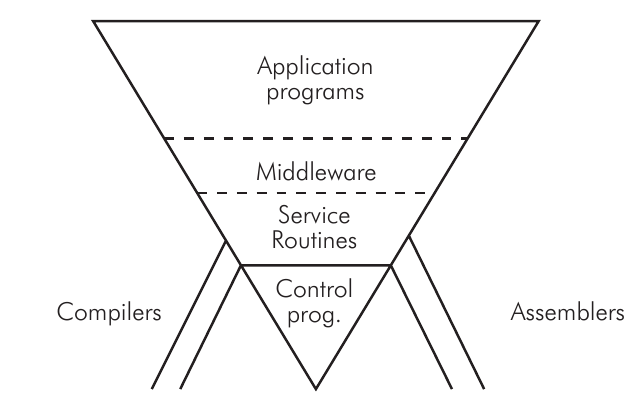
\includegraphics[width=0.9\textwidth]{figs/chapter2/software_pyramid.png}
    \caption{Organizzazione del software in esecuzione su un calcolatore generico.}
    \label{fig:sw_pyramid}
\end{figure}

L'idea è che un sistema complesso, così come una piramide invertita, non può restare operativo senza un adeguato supporto offerto da strumenti secondari, magari totalmente invisibili all'utente finale, ma che sono d'importanza vitale per il corretto funzionamento del tutto: \emph{compilatori} e \emph{assemblatori}, ossia programmi che traducono codice scritto in un qualche linguaggio prima nell'assembly dell'architettura target e poi in linguaggio macchina binario, tipicamente generando alla fine della pipeline di processamento un file eseguibile. Questi devono essere affidabili ed efficienti, poiché da essi dipende l'implementazione di tutto il resto.\\
Successivamente troviamo gli strati dei \emph{Control programs} e \emph{Service Routines}: si tratta di quelli che al giorno d'oggi siamo abituati a chiamare \emph{Sistema Operativo} e \emph{drivers}: questi vengono sviluppati solitamente a diretto contatto con la macchina, tenendone presenti le specificità, e dipendono fortemente dagli strumenti di compilazione impiegati. Il loro ruolo è quello di fornire un'astrazione dell'hardware che ne renda semplice l'utilizzo sia da parte dell'utente finale, che usa le applicazioni, sia da parte degli stessi programmatori di applicazioni. Ed il software applicativo è proprio quello che ritroviamo nell'ultimo livello: programmi che usano l'hardware più o meno direttamente per offrire agli utenti svariati servizi.\\
C'è però uno strato, intermedio, che solitamente non viene considerato poiché in passato non sempre presente o difficile da caratterizzare: il \emph{middleware}. Posizionato a metà tra il software di sistema e quello applicativo, il middleware trova la sua prima definizione e caratterizzazione proprio in occasione della suddetta conferenza. Inizialmente pensato solo come uno strato connettivo tra software corrente e \emph{legacy}, è un software che fornisce servizi e funzionalità comuni alle applicazioni al di fuori di quanto offerto dal sistema operativo. Dal punto di vista di quest’ultimo, si presenta come un normale software applicativo, composto ad esempio da librerie condivise o dinamiche. La gestione dei dati, i servizi applicativi, la messaggistica, l'autenticazione e la gestione delle API sono tutti compiti comunemente assolti dal middleware, il quale dunque aiuta gli sviluppatori a creare applicazioni in modo più efficiente, agendo come tessuto connettivo tra queste ultime, i dati e gli utenti.\newpage
In ambienti distribuiti o in presenza di container\footnote{Un \emph{container} è un pacchetto di software autosufficiente, comprendente sia il proprio codice sorgente che tutte le dipendenze, dunque pronto per essere direttamente eseguito su qualunque sistema o macchina. Sono spesso usati in ambienti virtualizzati, assegnandogli in parallelo porzioni delle risorse della macchina host e isolandogli tra loro, garantendo prestazioni uniformi e predicibili e il rispetto di standard di sicurezza.}, il middleware può rendere facile e conveniente sviluppare ed eseguire applicazioni su larga scala. Un servizio generalmente offerto da un middleware è un modo per scambiare dati tra applicazioni, anche tramite dispositivi diversi, secondo un formato comune denominato \emph{interfaccia} definito al bisogno.\\
In generale, i servizi offerti sono specificati solo nei termini della loro dinamica ma possono essere portati su diverse architetture e dispositivi, funzionandovi allo stesso modo pur mantenendo la loro implementazione nascosta all’utente finale: ad esempio, quando un middleware si occupa di realizzare la comunicazione tra applicazioni, in uno stack di rete si porrebbe tra il livello di trasporto e quello di applicazione.\\
Oggi, il middleware si può dividere in due tipologie: quello che opera in \emph{tempo umano}, e dunque è pensato per essere usato direttamente da utenti umani (e.g. servizi web), e quello che opera in \emph{tempo macchina}, ed è dunque composto principalmente da API che i programmatori di applicazioni possono usare per svolgere i loro compiti con più facilità e beneficiando di una maggiore portabilità verso un'ampia varietà di dispositivi.\\
Alla luce di tutto ciò, ricordando le difficoltà che comunemente si incontrano durante il design del software di un sistema robotico, ci si può rendere conto di come l'adozione di un middleware nei sottosistemi di più alto livello possa rendere le cose più semplici: molti dei moduli che andrebbero realizzati ex novo sarebbero invece implementati dal middleware stesso e offerti sotto forma di servizi da includere nei programmi da sviluppare.\vfill\newpage
